\documentclass{standalone}
\usepackage{tikz}
\usepackage{ctex,siunitx,ninecolors}
\setCJKmainfont{Noto Serif CJK SC}
\usepackage{tkz-euclide}
\usepackage{amsmath}
\usepackage{wasysym}
\usetikzlibrary{patterns, calc}
\usetikzlibrary {decorations.pathmorphing, decorations.pathreplacing, decorations.shapes}
\begin{document}
\small
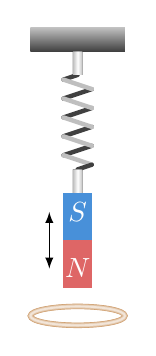
\begin{tikzpicture}[>=latex,scale=1.2]
  \fill[top color=lightgray,bottom color=darkgray](-0.5,0)rectangle(0.5,0.25);
  \draw[darkgray,line cap=round,ultra thick](0,-0.25)--(-0.15,-0.3);
  \foreach \x in {-0.3,-0.5,...,-1.0}
  {
    \draw[darkgray,line cap=round,ultra thick](0.15,\x-0.1)--(-0.15,\x-0.2);
    \draw[lightgray,line cap=round,ultra thick](-0.15,\x)--(0.15,\x-0.1);
  }
  \draw[lightgray,line cap=round,ultra thick](-0.15,-1.1)--(0.15,-1.2);
  \draw[darkgray,line cap=round,ultra thick](0,-1.25)--(0.15,-1.2);
  \fill[left color=lightgray,right color=lightgray,middle color=white](0.05,0)rectangle(-0.05,-0.25)(0.05,-1.5)rectangle(-0.05,-1.25);
  \fill[azure6](-0.15,-1.5)rectangle(0.15,-2.0);
  \fill[red6](-0.15,-2.5)rectangle(0.15,-2.0);
  \node at (0,-1.5)[below,text=white]{$S$};
  \node at (0,-2.5)[above,text=white]{$N$};
  \draw[<->](-0.3,-1.7)--(-0.3,-2.3);
  \foreach \x in {80,60,40,20}
  {
    \draw[line width={2*sin(\x)},brown!\x](0,-2.8)ellipse(0.5 and 0.1);
  }
\end{tikzpicture}
\end{document}